% Copyright Patrick Hall 2019
% CC by 4.0 license
% TODO: 
% - move conclusion to introduction
% - replace hypotheticals with examples, keep code in repo
% -- h2o-3 GBM DT + shapley; global shapley, resid analysis
% -- on PAY_0 being too important -- dont trust it
% - reintroduce model debugging and define roughly
% - publish on medium  


\documentclass[fleqn]{article}

\renewcommand\refname{}

\title{On Unhelpful Explainable Machine Learning Misconceptions}

\author{
  Patrick Hall\footnote{H2O.ai and George Washington University} \footnote{\copyright \hspace{1pt} Patrick Hall 2019. This work in progress is shared under a CC by 4.0 license.}\\
  Washington, DC\\
  \texttt{patrick.hall@h2o.ai}
}

\usepackage{graphicx}
\usepackage{fullpage}
\usepackage{pdfpages}
\usepackage{amsmath}
\usepackage{amssymb}
\usepackage{mathtools}
\usepackage{MnSymbol}
\usepackage{enumerate}
\usepackage{setspace}
\usepackage[colorlinks]{hyperref}
\usepackage{breakurl}
\usepackage{float}
\usepackage{caption}
\usepackage{subcaption}
\usepackage{multicol}
\usepackage{color}
\usepackage{listings}
\usepackage{csvsimple}
\usepackage{algorithm}
\usepackage{algorithmic}
\usepackage{verbatim}
\usepackage{mdframed}
\usepackage{changepage}
\usepackage[top=1in, bottom=1in, left=1in, right=1in]{geometry}

\begin{document}

\maketitle

\section*{Introduction}

As someone who has been involved in the implementation of explainable machine learning (ML) software for the past three years, I find a lot of what I read about the topic confusing and detached from my personal, hands-on experiences. This short text presents arguments, proposals, and references to address explainable ML misconceptions. Please note that this text is not an attack on any party. However, it does promote informed debate, scrutiny, and continued development of explainable ML, and not dismissal or derision of the discipline. Due to obvious community and customer demand, explainable ML methods have already been implemented in popular open source software and in commercial software.\footnote{Like h2o-3, xgboost, and various other Python and R packages. See: \url{https://github.com/jphall663/awesome-machine-learning-interpretability} for a longer, curated list of open source software packages.}\textsuperscript{,}\footnote{For instance  Datarobot, H2O Driverless AI, SAS Visual Data Mining and Machine Learning, Zest AutoML, and likely several others.} The methods will likely be used widely and proper usage discussions are probably more helpful than ``please stop'' requests \cite{please_stop}. Moreover, this text builds the seemingly natural case for a holistic approach to ML that includes interpretable (i.e ``white-box'') models along with explanatory, debugging, and disparate impact analysis and remediation techniques. Much groundbreaking work has been done in several related disciplines to make machine learning more interpretable and trustworthy, and the cursory application of traditional black-box ML to human-centered problems is now an outdated, ethically problematic, and potentially dangerous practice.\\

%``Please stop doing explainable machine learning,'' extolled one of the brightest minds in machine learning (ML) with the title of a recent and well-reasoned essay \cite{please_stop}. A related and admittedly-controversial short talk also included points such as, ``[Explainable ML] forces you to rely on two models instead of one,'' and argued that explainable machine learning can be a foil for companies and governments to conduct unsavory or negligent deeds with black-box models.\footnote{Statistics at a Crossroads, Webinar 2. URL: \url{https://zoom.us/recording/play/0y-iI9HamgyDzzP2k_jiTu6jB7JgVVXnjWZKDMbnyRTn3FsxTDZy6Wkrj3_ekx4J?startTime=1538497702000}} Perhaps even more noteworthy was the online response, which included musings such as, ``don’t forget hidden assumptions for explainable ML (e.g., locally linear behavior near predictions),'' and lamentations like, ``no one has explained to me what 'explainable' or 'interpretable' is.'' \footnote{Twitter thread: \url{https://twitter.com/tdietterich/status/1052680788389507073}} This article aims to clear up such misconceptions and fill the gaps in community knowledge exposed by these sentiments. Strangely, neither the talk nor the follow-up discussions seemed to allow for combining white-box models and post-hoc explanatory techniques. 

\begin{figure}[htb]
	\begin{center}
		\includegraphics[scale=0.33]{img/figure_1.png}
		\caption{An augmented learning problem diagram in which several post-hoc techniques create explanations for a credit scoring model $g$. When used properly, explanations can increase understanding of $g$ and help improve the accuracy, fairness, interpretability, privacy, or security of subsequent applications of $\mathcal{H}$ and $\mathcal{A}$. Adapted from Figure 1.2 of the open textbook \textit{Learning From Data} \cite{lfd}.}
		\label{fig:learning_problem}
	\end{center}
\end{figure}	

To avoid ambiguity, several initial internal definitions and accompanying examples are outlined before discussing misconceptions. As illustrated in Figure \ref{fig:learning_problem}, here \textit{explainable ML} means post-hoc techniques used to understand trained model behavior or predictions. Examples of common explainable ML techniques include:

\begin{itemize}
\item Local and global feature importance methods, in particular Shapley values \cite{shapley1988shapley}, \cite{keinan2004fair}, \cite{kononenko2010efficient}, \cite{shapley}.
\item Local and global model-agnostic surrogate models, such as surrogate decision trees and Local Interpretable Model-agnostic Explanations (LIME) \cite{dt_surrogate1}, \cite{dt_surrogate2}, \cite{lime-sup}, \cite{lime}. 
\item Local and global visualizations of model predictions such as accumulated local effect (ALE), 1- and 2-dimensional partial dependence, and individual conditional expectation (ICE) plots \cite{ale_plot}, \cite{esl}, \cite{ice_plots}.
\end{itemize}  

\noindent In this text \textit{model debugging} refers to testing ML models to increase trust in model mechanisms and predictions. Examples of model debugging techniques include variants of sensitivity (i.e. ``what-if?'') and residual analysis used to test models for errors or security vulnerabilities. Model debugging should also include remediating any discovered errors or vulnerabilities. Herein \textit{fairness} techniques refer to canonical disparate impact analysis, model selection by minimization of disparate impact, and remediation techniques such as disparate impact removal preprocessing or equalized odds post processing \cite{feldman2015certifying}, \cite{hardt2016equality}. In this text \textit{interpretable} or \textit{white-box} models will include linear models, decision trees, constrained or Bayesian variants of traditional black-box ML models, or novel types of models designed to be directly interpretable. Additional examples of interpretable modeling techniques include explainable neural networks (XNNs), monotonically constrained gradient boosting machines (GBMs)\footnote{As implemented in XGBoost (\url{https://xgboost.readthedocs.io/en/latest/tutorials/monotonic.html}) or H2O-3 (\url{https://github.com/h2oai/h2o-3/blob/master/h2o-py/demos/H2O_tutorial_gbm_monotonicity.ipynb}).}, scalable Bayesian rule lists, or super-sparse linear integer models (SLIMs) \cite{wf_xnn}, \cite{sbrl}, \cite{slim}. Herein unconstrained, traditional black-box ML models, such as multilayer perceptron (MLP) neural networks and GBMs, are said to be uninterpretable. 

\section{Misconception: Explanations are Necessary and Sufficient to Establish Trust in ML}

Explanations are likely necessary for trust in many cases, but certainly not sufficient for trust in all cases. 
Explanation, as a general concept, is related more directly to understanding and transparency than to trust.\footnote{The Merriam-Webster definition of \textit{explain}, accessed April 21\textsuperscript{st} 2019, does not mention \textit{trust}} Simply put, one can understand and explain something without trusting it. One can also trust something and not be able to understand or explain it. Consider the following example scenarios:

\begin{itemize}

\item \textbf{Explanation and understanding without trust}: In Figure \ref{fig:figure_2}, global Shapley explanations and residual analysis identify a pathology in an unconstrained GBM model, $g_{\text{GBM}}$. $g_{\text{GBM}}$ over emphasizes the input feature \texttt{PAY\_0}, or a customer's most recent repayment status. Over-weighing \texttt{PAY\_0} makes $g_{\text{GBM}}$ often unable to predict on-time payment if recent payments are delayed (\texttt{PAY\_0} $>$ 1), causing large negative residuals. $g_{\text{GBM}}$ is also often unable to predict default if recent payments are on-time (\texttt{PAY\_0} $leq$ 1), causing large positive residuals. In this example scenario, $g_{\text{GBM}}$ is explainable, but not trustworthy. 

\begin{figure}
\begin{subfigure}{.5\textwidth}
  %\centering
  \includegraphics[width=.84\linewidth]{img/figure_2a.png}
  \caption{Global Shapley feature importance values for $g_{\text{GBM}}$.}
  \label{fig:2a}
\end{subfigure}%
\begin{subfigure}{.5\textwidth}
  \centering
  \includegraphics[width=1.1\linewidth]{img/figure_2b.png}
  \caption{$g_{\text{GBM}}$ deviance residuals and predictions by \texttt{PAY\_0}.}
  \label{fig:2b}
\end{subfigure}
\label{fig:figure_2}
\caption{An unconstrained GBM probability of default model, $g_{\text{GBM}}$, over-emphasizes the importance of the input feature \texttt{PAY\_0}, a customer's most recent repayment status. $g_{\text{GBM}}$ produces large positive residuals when \texttt{PAY\_0} indicates on-time payments and large negative residuals when \texttt{PAY\_0} indicates late payments.}
\label{fig:figure_2}
\end{figure}

\item \textbf{Trust without explanation and understanding}: Years before reliable explanation techniques were widely acknowledged and available, black-box predictive models, such as autoencoder and MLP neural networks, were used for fraud detection in the financial services industry \cite{gopinathan1998fraud}. When these models performed well, they were trusted.\footnote{For example: \url{https://www.sas.com/en_ph/customers/hsbc.html}, \url{https://www.kdnuggets.com/2011/03/sas-patent-fraud-detection.html}.} However, they were not explainable or well-understood by contemporary standards.  

\end{itemize}

If trust in models is your goal, then explanations alone are not sufficient. However, as discussed in Section \ref{sec:white_box} and illustrated in Figure \ref{fig:hc_ml}, in an ideal scenario, explanation techniques would be used with a wide variety of other methods to increase accuracy, fairness, interpretability, privacy, security, and trust in ML models. 

\section{Misconception: Explainable ML is Unnecessary}

Local feature importance values for negative credit decisions, i.e. adverse action codes, are mandated under the Fair Credit Reporting Act for many credit lending decisions in the United States. If machine learning is used for such decisions, it has to be explained with local feature importance. In a number of other application domains, broader interpretability is also legal necessity. Explanation, along with white-box models, model debugging, disparate impact analysis, and the documentation they enable, can also be required under the Civil Rights Acts of 1964 and 1991, the Americans with Disabilities Act, the Genetic Information Nondiscrimination Act, the Health Insurance Portability and Accountability Act, the Equal Credit Opportunity Act, the Fair Housing Act, Federal Reserve SR 11-7, the European Union (EU) Greater Data Privacy Regulation (GDPR) Article 22, and other regulatory statutes \cite{ff_interpretability}.

\section{Misconception: All the Key Terms in Explainable ML are Undefined}

Helpful definitions that apply to explainable ML have been put forward, including:

\begin{itemize}
\item \textbf{Interpretable}: ``The ability to explain or to present in understandable terms to a human'' -- in ``Towards a Rigorous Science of Interpretable Machine Learning'' by Doshi-Velez and Kim (2017) \cite{been_kim1}.
\item \textbf{A Good Explanation}: ``When you can no longer keep asking why'' -- in ``Explaining Explanations: An Approach to Evaluating Interpretability of Machine Learning'' by Gilpin et al. (2018) \cite{gilpin2018explaining}. (Gilpin et al. also provide several clear constructs for describing more specific types of explanations.) 
\end{itemize}



While the explainable ML field is far from embracing a clear and accepted taxonomy of concepts or an exhaustive and precise vocabulary, these two well-founded definitions appear to link explanations to some ML process being interpretable. Moreover, many authors have made significant attempts to grapple with a variety of general concepts related to interpretability and explanations, including ``A Survey Of Methods For Explaining Black Box Models'' by Guidotti et al. (2018), Zachary Lipton's ``The Mythos of Model Interpretability'' (2016), Christoph Molnar's \textit{Interpretable Machine Learning} (2018), and Adrian Weller's ``Challenges for Transparency'' (2017) \cite{guidotti2018survey},  \cite{lipton1}, \cite{molnar}, \cite{weller2017challenges}. 

\section{Misconception: Explainable ML is Just Models of Models}

Models of models, or surrogate models, can be helpful explanatory tools, but they are usually approximate, low-fidelity explainers. Aside from 1.) a global summary of a complex model provided by a surrogate model can be helpful sometimes and 2.) much work in explainable ML has been directed toward improving the fidelity and usefulness of surrogate models \cite{dt_surrogate1}, \cite{dt_surrogate2}, \cite{lime-sup}, \cite{wf_xnn}, \textbf{many explainable ML techniques have nothing to do with surrogate models!}   

One of the most exciting breakthroughs for supervised learning problems in explainable ML is the application of a coalitional game theory concept, Shapley values, to compute feature contributions which are consistent globally and accurate locally using the trained model itself \cite{kononenko2010efficient}, \cite{shapley}. An extension of this idea, called tree SHAP, has already been implemented for popular tree ensemble methods \cite{tree_shap}. There are many other explainable ML methods that operate on trained models directly such as partial dependence and ICE plots \cite{esl}, \cite{ice_plots}. Notably, surrogate models and explanatory techniques that operate directly on trained models can be combined, for instance by using partial dependence, ICE, and surrogate decision trees to investigate and confirm modeled interactions \cite{art_and_sci}. 

For a curated list of many different types of white-box modeling techniques, and model-specific, model-agnostic, and surrogate model explainable ML techniques, please see:
\begin{center}
\url{https://github.com/jphall663/awesome-machine-learning-interpretability}
\end{center}

\textbf{Misconception Corollary: Explainable ML is just LIME.} LIME, in it's most popular implementation, uses local linear surrogate models \cite{lime}. LIME is important, and imperfect, but just one of many explainable ML tools. And again, LIME can sometimes be combined with model-specific methods to yield deeper insights. Consider that tree SHAP can provide locally accurate and consistent point estimates for local feature importance whereas LIME can provide approximate information about modeled local linear trends around the same point.   

\section{Misconception: Explainable ML Methods Simply Provide Cover to Use Black-Box ML for Nefarious Purposes}

If used disingenuously, explainable ML methods probably do provide such cover \cite{fair_washing}. But explainable ML methods were designed specifically to crack open those same nefarious and complex black-boxes. See Angwin et al. (2016) for evidence that hacking or stealing of commercial black-box models for oversight purposes is possible \cite{angwin16}. Such investigations would likely only be improved by advances in explanatory and fairness tools. Additionally, many important computer-based technological advances present similar double-edged sword dilemmas, e.g. social media or strong encryption. Rarely does the ability of a tool to be misused for malicious purposes disqualify it from being used as designed. 

\section{Misconception: Explainable ML Methods and White-box Models are Somehow Mutually Exclusive} \label{sec:white_box}

A few well-known publications have focused either on white-box modeling techniques (e.g. \cite{slim}, \cite{sbrl}) or on post-hoc explanations (e.g. \cite{lime}, \cite{shapley}), but the two can be used together in the context of a broader and more human-centered machine learning workflow as illustrated in Figure \ref{fig:hc_ml}. 

\begin{figure}[htb]
	\begin{center}
		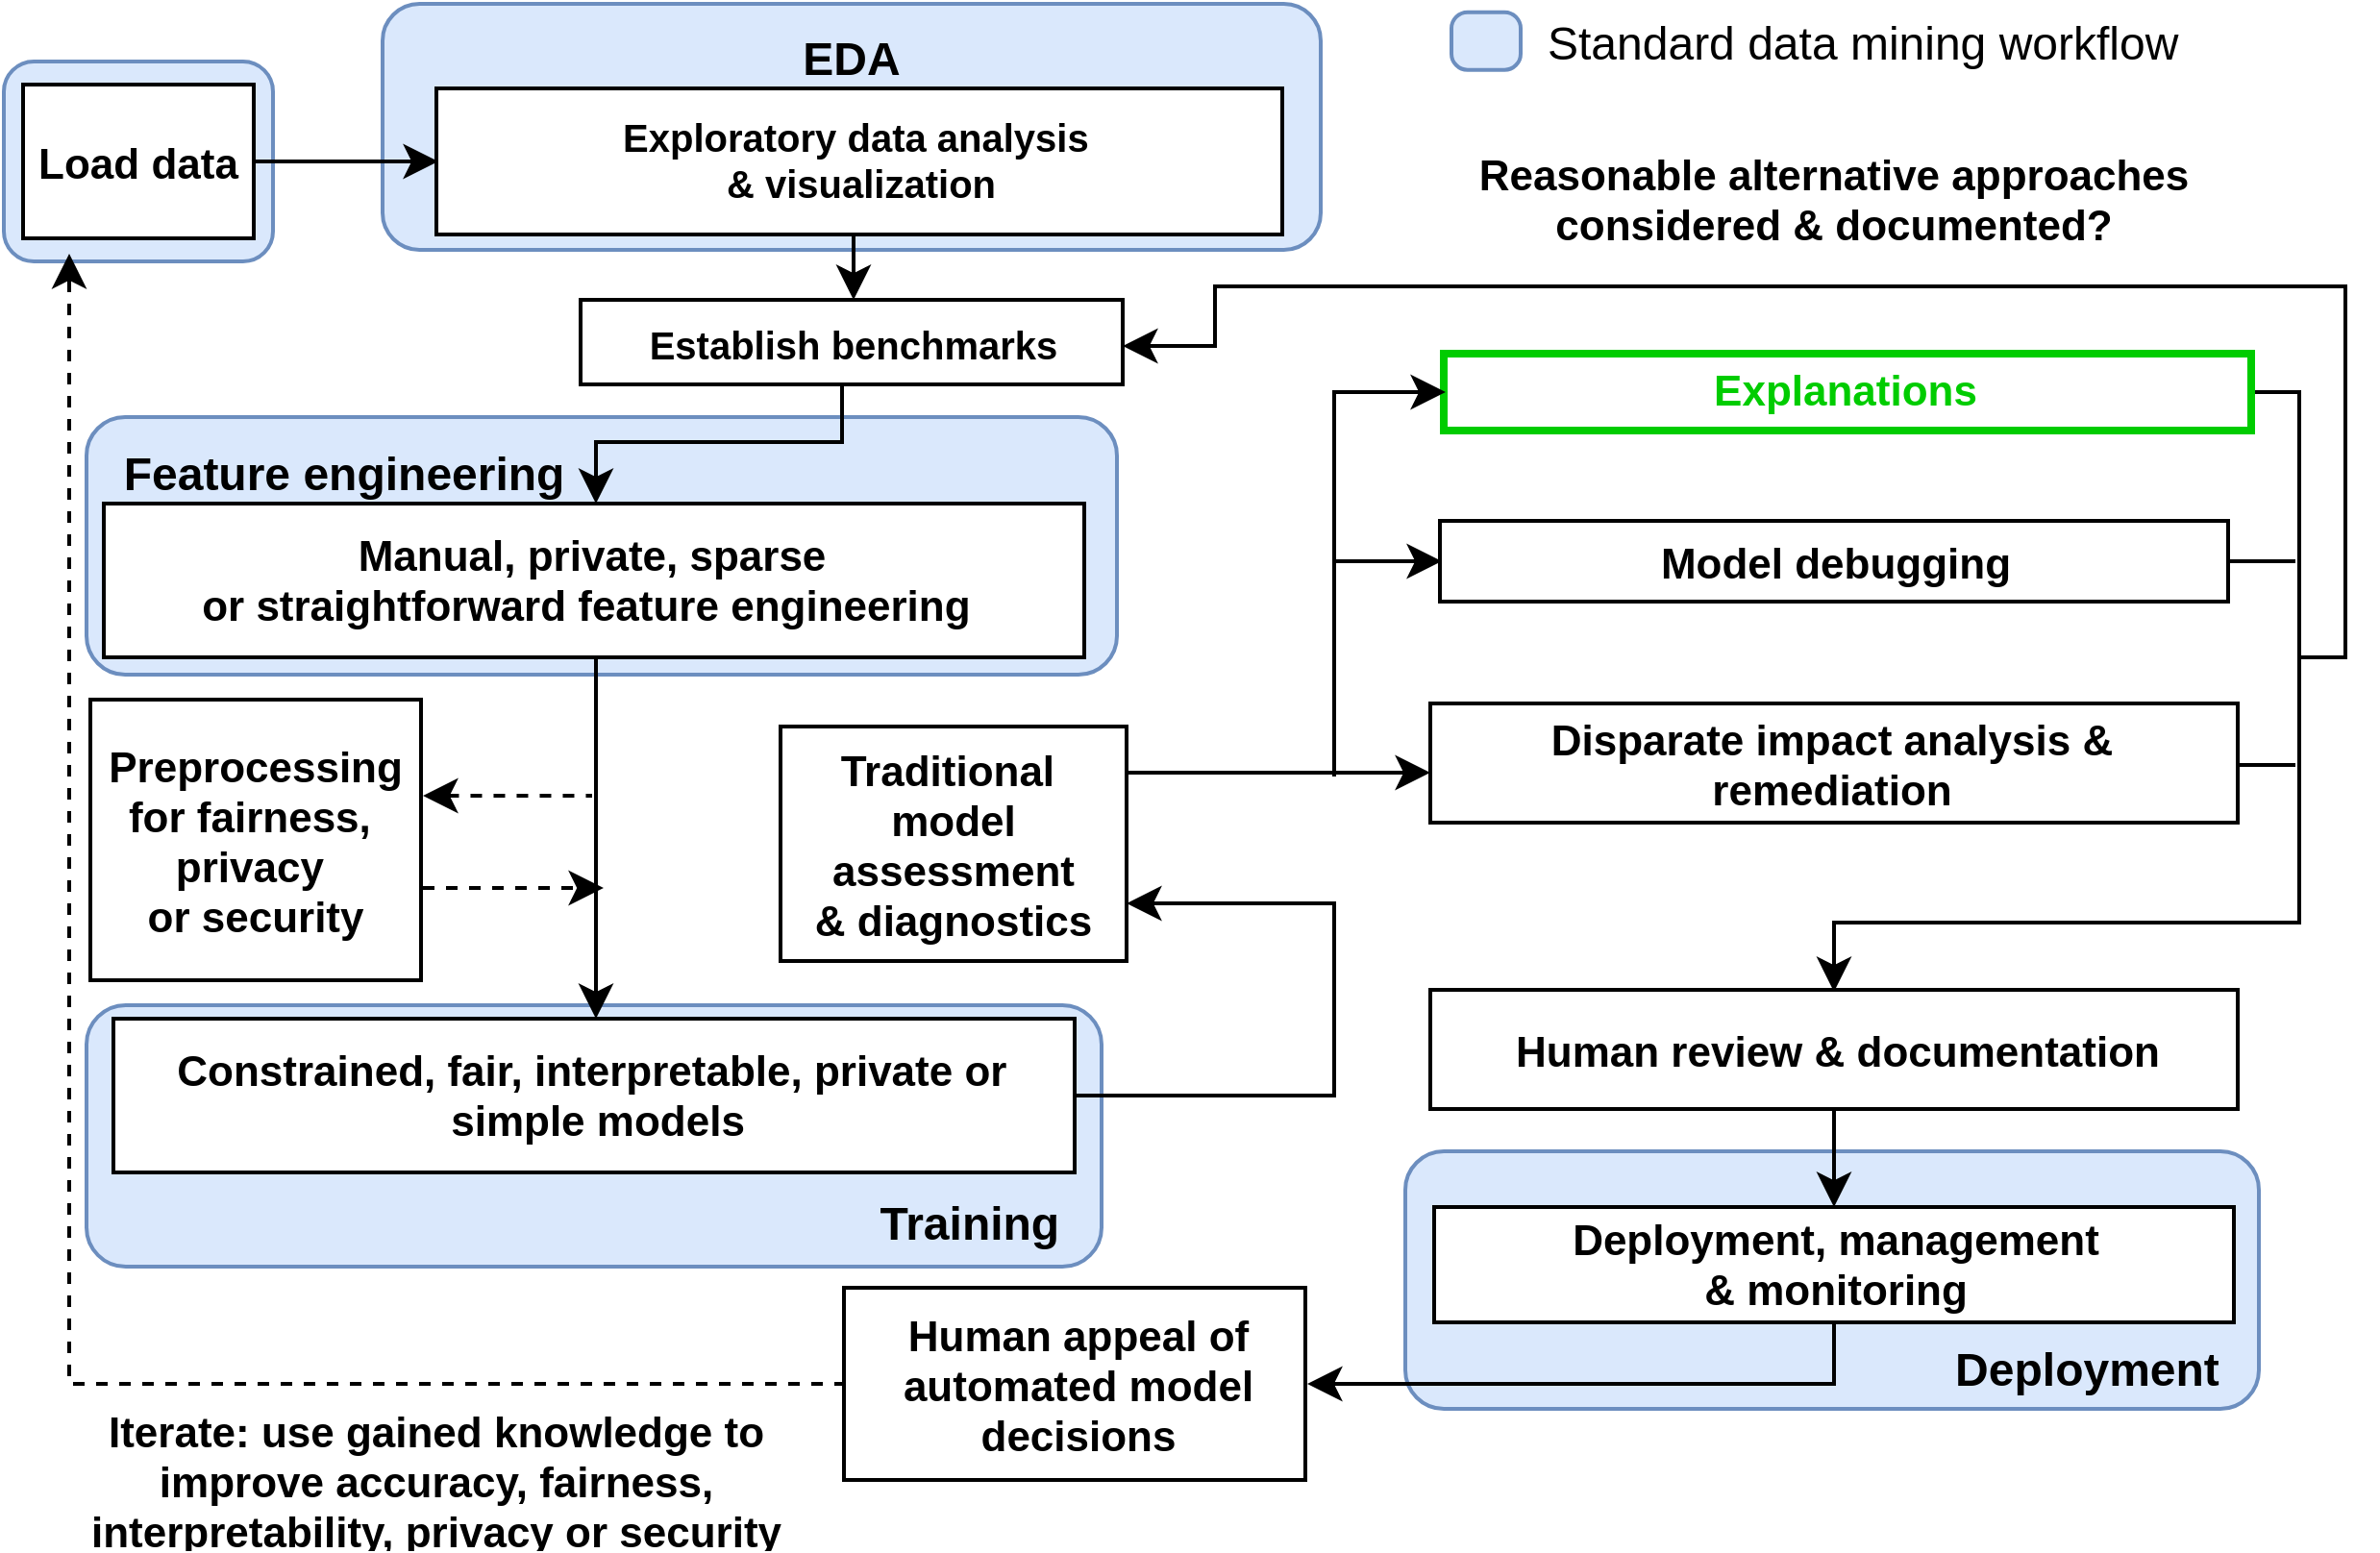
\includegraphics[scale=0.15]{img/figure_3.png}
		\caption{A diagram of a proposed human-centered machine learning workflow in which explanations (highlighted in green) are used along with interpretable models, disparate impact analysis and remediation techniques, and other review and appeal mechanisms to create a fair, accountable, and transparent ML system.}
		\label{fig:hc_ml}
	\end{center}
\end{figure}	

Consider the seemingly useful example case of augmenting globally interpretable models with local post-hoc explanations: A practitioner could train a single pruned decision tree as a globally interpretable model then use local explanations in the form of Shapley feature importance. This would enable the practitioner to see accurate numeric feature contributions for each model prediction in addition to the entire directed graph of the decision tree. Isn't a complete global and local understanding of the model more desirable than the white-box model or the post-hoc explanations alone?\\ 

\textbf{Corollary Misconception: Explainable ML Methods and Fairness Methods are Somehow Mutually Exclusive}: Like white-box models, fairness methods are often presented in different articles than post-hoc explanatory methods. However, in banks, using post-hoc explanatory tools such as partial dependence plots and local feature importance to comply with credit reporting regulations often goes hand-in-hand with using disparate impact analysis to comply with fair lending regulations. 

\section*{Conclusion}

%Machine learning systems are used today to make life-altering decisions about employment, bail, parole, and lending. The scope of decisions delegated to machine learning systems seems likely only to expand in the future. Unfortunately serious discrimination, privacy, and even accuracy concerns can be raised about these systems. Many researchers and practitioners are tackling disparate impact, inaccuracy, privacy violations, and security vulnerabilities with a number of brilliant, but often siloed, approaches. This short text illustrates how to combine innovations from several sub-disciplines of machine learning research to train explainable, fair, trustable, and accurate predictive modeling systems. Together these techniques can create a new and truly human-centered type of machine learning suitable for use in business- and life-critical decision support.

\section*{Acknowledgemnts}

The author thanks Pramit Choudhary and Navdeep Gill at H2O.ai for their input and insights. 

%-------------------------------------------------------------------------------
\section*{References}
%-------------------------------------------------------------------------------
\bibliographystyle{plain}
\bibliography{xai_misconceptions}

\end{document}

% let doug proofread